Machine indexing of institutional repositories: indexing Edoc with Annif
and BARTOC FAST as proof of concept

\hypertarget{introduction}{%
\section{Introduction}\label{introduction}}

\hypertarget{outline}{%
\subsection{Outline}\label{outline}}

\hypertarget{method}{%
\subsection{Method}\label{method}}

!! Say something to the effect that all data and code are available on
GitHub.

\hypertarget{tools-and-configuration}{%
\subsection{Tools and configuration}\label{tools-and-configuration}}

\hypertarget{openrefine}{%
\subsubsection{OpenRefine}\label{openrefine}}

For data refinement I use OpenRefine version 3.4.1
(https://openrefine.org/). Data manipulation in OpenRefine is tracked:
the manipulation history of some data can be exported as JSON file and
then reproduced (on the same data on a different machine or on different
data) by loading said file. I will supply a corresponding manipulation
history whenever appropriate. Note that when using OpenRefine with
larger files (and there are many such files in this project), the memory
allocation to OpenRefine must be manually increased (see
https://docs.openrefine.org/manual/installing/\#increasing-memory-allocation
for details).

\hypertarget{prototype}{%
\section{Prototype}\label{prototype}}

In this chapter, the prototype for a machine indexing of Edoc is
presented. The focus is primarily on practical implementation although
care is taken to spell out design decisions in as much detail as is
needed.

\hypertarget{aim}{%
\subsection{Aim}\label{aim}}

Let us start by stating the aim of the prototype. From a functional
perspective, the prototype takes a subset of the data from Edoc as input
and provides index terms for each item in this subset as output. In
order to fulfill this aim we can distinguish a number of steps that need
to be taken:

\begin{enumerate}
\def\labelenumi{\arabic{enumi}.}
\tightlist
\item
  Understand the Edoc data.\\
\item
  Select and construct a sample data set.
\item
  Use Annif to index the items in the sample data set.
\item
  Construct a gold standard from the keywords.
\item
  Assess the quality of the output based on the gold standard.
\end{enumerate}

In the sections below, these steps will be discussed in detail.

\hypertarget{edoc-data}{%
\subsection{Edoc data}\label{edoc-data}}

\hypertarget{edoc}{%
\subsubsection{Edoc}\label{edoc}}

Edoc is the institutional repository of the University of Basel. It was
conceived in 2009 as repository for electronic dissertations and grew in
scope when the University of Basel adapted its first open access policy
in 2013. As per today Edoc contains roughly 68'000 items.

Edoc runs on the EPrints 3 document management system
(https://github.com/eprints/eprints).\\
!! Add technical description of Edoc.\\
!! Perhaps add description of how files are added to Edoc, see PDF in
\texttt{/todo}.

\hypertarget{data-extraction}{%
\subsubsection{Data extraction}\label{data-extraction}}

Even though Edoc is a public server, its database does not have a
web-ready API. In addition, since Edoc is a production server, its
underlying database cannot be used directly on pain of disturbing the
provided services. The data hence needs to be extracted from Edoc in
order to work with it. This could for example be achieved by cloning the
database of the server and running it on a local machine. However, this
route was not available due to the limited resources of the responsible
co-workers. I thus employed a workaround: Edoc has a built-in advanced
search tool where the results can be exported. Even though it is not
possible to extract all database items by default, only one of the many
available search fields has to be filled in. The complete database can
hence be extracted by only filling in the \texttt{Date} field and using
a sufficiently permissive time period such as 1940 to 2020 since the
oldest record in the database was published in 1942. On January 21 2021,
this query yielded 68'345 results. These results were then exported as a
326 MB JSON file called \texttt{1942-2020.json}. \texttt{1942-2020.json}
has two drawbacks. First, the maximum file size on GitHub is 100 MB. And
second, \texttt{1942-2020.json} is too big to be handled by standard
editors requiring special editors such as Oxygen. For these reasons
\texttt{1942-2020.json} was split into smaller files that are easier
handled and can be uploaded to GitHub. For this
\texttt{\_Utility.split\_json} was used yielding 14 files of size 20 MB
or less containing 5000 or fewer entries each. These files are called
\texttt{raw\_master\_x-y.json} (where x and y indicate the entries as
given by \texttt{1942-2020.json}) and saved under \texttt{/edoc/raw}.

\hypertarget{data-description-and-analysis}{%
\subsubsection{Data description and
analysis}\label{data-description-and-analysis}}

!! Explain the Edoc data fields. Say perhaps something about the
granularity of the relevant fields. Say something about how the fields
are filled in (and by whom).

\hypertarget{sample-data-set}{%
\subsection{Sample data set}\label{sample-data-set}}

In this section, I will explain how the sample data set is selected and
constructed. ``Selection'' means the task of specifying a subset of the
Edoc data and ``construction'' means the task of implementing this
selection.

\hypertarget{selection}{%
\subsubsection{Selection}\label{selection}}

There are a number of constraints for selecting the sample data set
pertaining to an items's text, evaluability and the data set's scope.

The first constraint stems from Annif, the machine indexing framework
that will be used. Put simply, machine indexing assigns index terms to a
text based on training data. The training data consists of a set of
texts, a vocabulary, and function from vocabulary to texts. In this
context we mean by ``text'' a sequence of words in a natural language
and by ``vocabulary'' a set of words. Intuitively, the training data
consists of pairs of text and subject terms that meet some standard. The
training data and the vocabulary are already supplied by Annif, we only
need to provide a text for each item that we want to be assigned index
terms. Therefore, we only select items with text.

The second constraint is that we must be able to evaluate the quality of
the index terms assigned by Annif to any item in the sample data set.

The third and final constraint takes into account the possibility of
having to extend the prototype to the complete Edoc data. On the one
hand, the sample data set should be small enough to allow for easy
handling and rapid iteration. On the other hand, the sample data set
should not be trivial but reflect the quirks and inadequacies of the
complete dataset. In other words, we are looking for an abstraction
rather than an idealization in the sense of Stokhof and van Lambalgen
(2011).

\hypertarget{construction}{%
\subsubsection{Construction}\label{construction}}

The first constraint is that each item in the sample data set needs to
have a text. Intuitively, this text could consist of a title, an
abstract, or even a full text, or any combination of the above. Similar
to manual indexing, having more information (that is, longer texts)
usually implies a higher indexing quality in machine indexing. However,
this assumption needs to be confirmed empirically for the given machine
indexing framework and data set. If indeed confirmed, it might be
advisable only to index items that have a certain minimal text length.
Therefore, in order to construct the sample data set, we require each
item to have a non-empty value in the data fields \texttt{title},
\texttt{abstract}, and \texttt{id\_number} as proxy to retrieve a full
text remotely. Note that even more context could be provided by taking
into account other data fields such as \texttt{type},
\texttt{publication} or \texttt{department}. Especially the latter might
be valuable when disambiguating homonymous or polysemous words. For
example, consider the item
\texttt{https://edoc.unibas.ch/id/eprint/76510} which is titled
``Blacking Out.'' Without further context, this title could refer
(amongst others) to a physiological phenomenon, a sudden loss of
electricity, or a measure taken in wartime. Knowing that the item was
published by a researcher employed by the Faculty of Business and
Economics (and not, say, by the Faculty of Medicine) gives us reason to
exclude the first meaning. However, this idea cannot be implemented with
the out of the box instance of Annif employed in this chapter (see
\protect\hyperlink{machine-indexing}{subsection ``Machine indexing''}).

The second constraint is that the index terms assigned to each item in
the sample data set must be assessable. How the assessment is conducted
in detail is discussed in \protect\hyperlink{assessment}{section
``Assessment''}. For now, it is sufficient to say that we require a
standard against which we can evaluate the assigned index terms. By
``standard'' I mean that given a vocabulary of index terms and our
sample data set, for every item in the sample data set, there is an
approved subset of the vocabulary. The production of a standard from
scratch is of course is very costly since a person, usually highly
skilled in a certain academic domain, must assign and/or approve each
item's index terms (!!source). For this reason we try to avoid having to
produce a standard. One way of doing so is by requiring items in the
sample data set to have non-empty \texttt{keywords} data field. The
caveats of this approach are discussed in
\protect\hyperlink{assessment}{section ``Assessment''}.

Taking into account the third constraint simply means that we do not
employ any further restrictions. We can hence construct the sample data
set by choosing exactly those items from \texttt{/edoc/raw} which have
non-empty data fields \texttt{title}, \texttt{abstract},
\texttt{id\_number}, and \texttt{keywords}. We do so by calling
\texttt{\_Data.select\_from\_file} iteratively for all files in
\texttt{/edoc/raw}. The resulting file is saved in
\texttt{/edoc/selected} as \texttt{selected\_master.json}.

\hypertarget{analysis}{%
\subsubsection{Analysis}\label{analysis}}

Of the 68'345 items in \texttt{/edoc/raw}, all have a title (non-empty
\texttt{title} data field), a little more than half of the items have an
abstract (37'381 items with non-empty \texttt{abstract} data field),
roughly half of the items have an ID (35'355 items with non-empty
\texttt{id\_number} data field),\footnote{Note that when using the facet
  by blank on \texttt{id\_number} in OpenRefine, there are 57'153
  matches; this is due to the fact that many items with an ID such as
  DOI have secondary or tertiary IDs such as ISI or PMID.} and less than
10\% of the items have keywords (6'660 items with non-empty
\texttt{keywords} data field). The sample data set as requires all the
above data fields to be non-empty;
\texttt{/edoc/sample/sample\_master.json} has 4'111 items and hence
constitutes 6\% of the raw data.

In order to determine how well the sample data set represents the raw
Edoc data, a one-sample chi-square test was conducted on each selection
data field (see Parke 2013, chap. 1). The results indicate that the
sample data proportions of items are significantly different from the
raw Edoc data per department (see Figure 1 for more details).

\begin{figure}
\centering
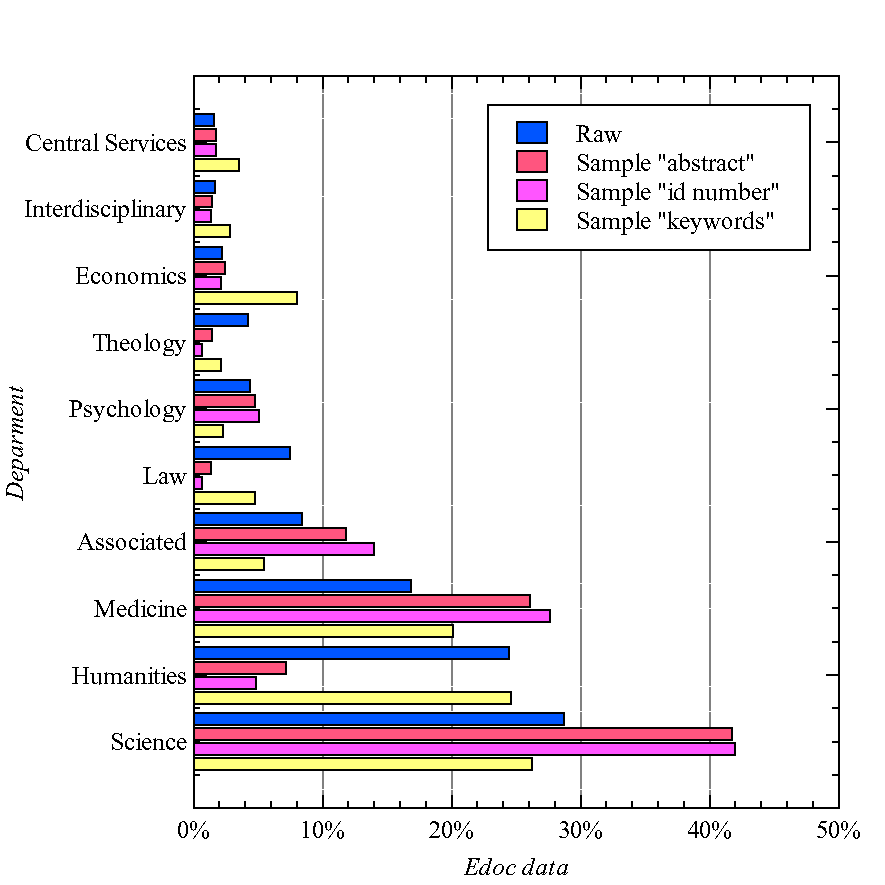
\includegraphics{images/chi_square_selection_fields.pdf}
\caption{The sample data set (\(n\) = 4'111) is not representative of
the raw Edoc data (\(n\) = 68'345) per department. Data field
\texttt{abstract}: \(\chi^2 (df=9) =\) 3'160.556, \(p < 0.001\); data
field \texttt{id\_number}: \(\chi^2 (df=9) =\) 4'209.0285,
\(p < 0.001\); data field \texttt{keywords}: \(\chi^2 (df=9) =\)
2'314.533, \(p < 0.001\). The data foundation is available at
\texttt{/edoc/analysis} and the chi-square statistic can be calculated
by calling \texttt{\_Analysis.chi\_square\_fit}.}
\end{figure}

The sample data set is hence not representative of the raw Edoc data.
This is not surprising since its construction is strongly biased. This
bias has the effect that the sample data set is significantly skewed
towards English journal publications in the sciences, medicine and
economics from the 21st century (see Figure 2 for more details). The
upshot of this analysis is that the humanities are underrepresented in
the sample data set. Therefore, any results with respect to the quality
of machine indexing discussed below might not be applicable to the
humanities.

\begin{figure}
\centering
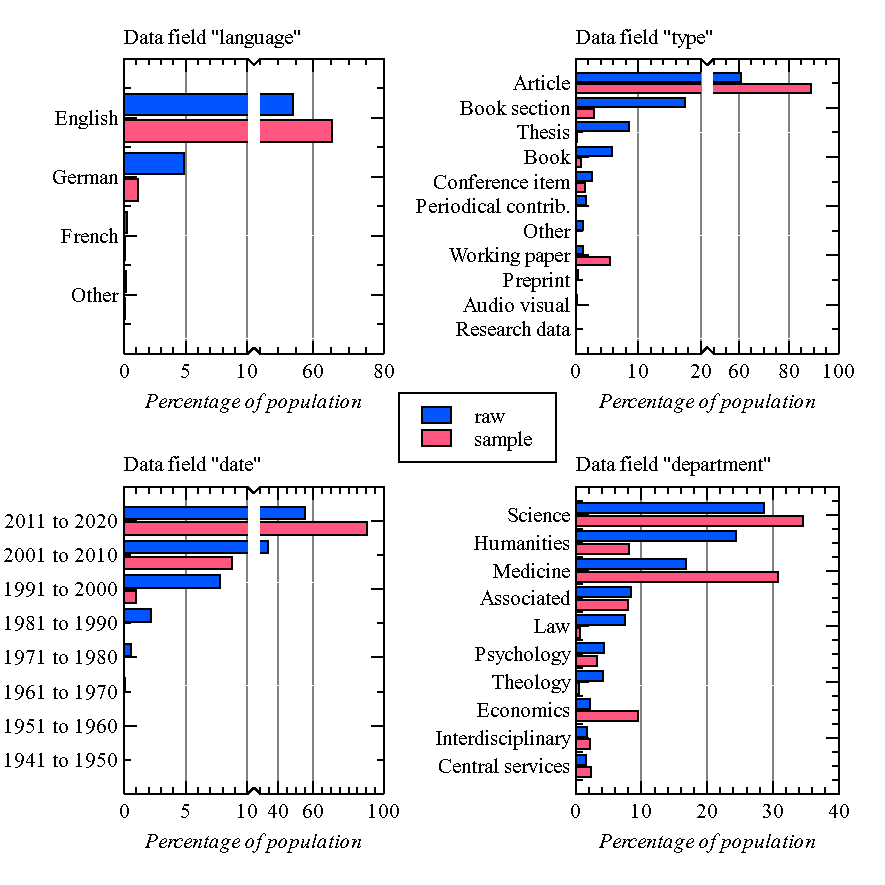
\includegraphics{images/raw_sample_analysis.pdf}
\caption{The sample data set (\(n\) = 4'111) is significantly skewed
towards English (data field \texttt{language}: \(\chi^2 (df=3) =\)
1'441.414, \(p < 0.001\)) journal publications (data field
\texttt{type}: \(\chi^2 (df=10) =\) 52'519.743, \(p < 0.001\)) in the
sciences, medicine and economics (data field \texttt{department}:
\(\chi^2 (df=9) =\) 14'447.276\$, \(p < 0.001\)) from the 21st (data
field \texttt{date}: \(\chi^2 (df=7) =\) 35'878.493, \(p < 0.001\))
century as compared to the raw Edoc data (\(n\) = 68'345). The data
foundation is available at \texttt{/edoc/analysis} and the chi-square
statistic can be calculated by calling
\texttt{\_Analysis.chi\_square\_fit}.}
\end{figure}

\hypertarget{machine-indexing}{%
\subsection{Machine indexing}\label{machine-indexing}}

\hypertarget{general-overview}{%
\subsubsection{General overview}\label{general-overview}}

!! Give an overview over machine indexing.

\hypertarget{annif}{%
\subsubsection{Annif}\label{annif}}

!! Given an intro to Annif. Explain that we are using the out of the box
version

\hypertarget{implementation}{%
\subsubsection{Implementation}\label{implementation}}

As explained above, for the prototype we will use the out

!! Explain how to implementation works.

In addition to the already used algorithms we should also try
https://ai.finto.fi/?locale=en

!! Somewhere here we talk about indexing based on title and/or abstract
and/or fulltext. Fulltext is not yet implemented. Some observations to
do so: - the link to the fulltext is constructed from the data fields
\texttt{offical\ url} and \texttt{documebts\ -\ main}, e.g.,
\texttt{https\ \ ://edoc.unibas.ch/79633/} + \texttt{1/} +
\texttt{2020\_18\_Informed\ by\ wet\ feet\_How\ do\ floods\ affect\ property\ prices.pdf}
to get
\texttt{https://edoc.unibas.ch/79633/1/2020\_18\_Informed\ by\ wet\ feet\_How\ do\ floods\ affect\ property\ prices.pdf}

\hypertarget{gold-standard}{%
\subsection{Gold standard}\label{gold-standard}}

In this chapter I will construct three distinct gold standards in order
to assess the quality of machine indexing the sample data set with
Annif.\\
!! Say something about assessments of Annif that have already been
carried out.

\hypertarget{definition}{%
\subsubsection{Definition}\label{definition}}

The most common approach for assessing the output of machine indexing is
by systematically comparing it with a gold standard (sometimes also
referred to as model or reference). Golub et al. (2016, 10) define a
gold standard as ``a collection in which each document is assigned a set
of {[}subject terms{]} that is assumed to be complete and correct''
where ``\emph{complete} means that all subjects that should be assigned
to a document are in fact assigned, and \emph{correct} means that there
are no subjects assigned that are irrelevant to the content.'' Put
inversely, if an item in the gold standard lacks subject terms
describing its content, the assignment is not complete; and if an item
in the gold standard has been assigned subject terms that are not
relevant to its content, the assignment is not correct.

A gold standard is usually the product of manual indexing by
``information experts, subject experts, or potential or real end users''
(Golub et al. 2016, 10). This entails its own host of epistemic problems
relating to objectivity and consistency of the assigned subject terms.
Most importantly, however, the construction of a gold standard from
scratch is very expensive. It is therefore not an option for the project
at hand. Rather, I will construct what could be called derivative gold
standards by reusing indexing data that is already available. Here we
can distinguish two distinct kinds of derivative gold standards: first,
I will construct a derivative gold standard based on the author keywords
available in the sample data set; call this the ``native'' gold
standard. Second, I will construct a derivative gold standard based on
indexing metadata available in repositories distinct from Edoc; call
this the ``foreign'' gold standard.

There are other methods for assessing machine indexing quality besides
comparison with a gold standard that are worth mentioning. These include
an evaluation in the context of indexing workflows (Golub et al. 2016,
13ff.), the assessment of retrieval performance (Golub et al. 2016,
15--23.), and so-called model free assessments (Louis and Nenkova 2013).

\hypertarget{native-gold-standard}{%
\subsubsection{Native gold standard}\label{native-gold-standard}}

The construction of the native gold standard takes x steps:

\begin{enumerate}
\def\labelenumi{\arabic{enumi}.}
\tightlist
\item
  Extract the keywords from the sample data set.\\
\item
  Clean the extracted keywords.
\item
  Reconcile the extracted keywords with\ldots{}
\end{enumerate}

The intended output of this transformation process is\ldots{}

These steps are explained in more detail in what follows.

\hypertarget{extract-keywords}{%
\paragraph{Extract keywords}\label{extract-keywords}}

In a first step, the keywords must be extracted from the sample data set
\texttt{/sample/sample\_master.json}. Recall that we mandated a
non-empty \texttt{keywords} data field for an item to be selected from
the raw Edoc data (see \protect\hyperlink{selection}{subsection
``Selection''}). We can thus simply copy the information in the
\texttt{keywords} data field on a per item basis. To do this, we call
\texttt{\_Keywords.extract\_keywords} with the sample data set as
argument and save the output as
\texttt{keywords/keywords\_extracted.json} like so:

\begin{Shaded}
\begin{Highlighting}[]
\NormalTok{keywords }\OperatorTok{=}\NormalTok{ \_Keywords.extract\_keywords(DIR }\OperatorTok{+} \StringTok{"/sample/sample\_master.json"}\NormalTok{)}
\NormalTok{\_Utility.save\_json(keywords, DIR }\OperatorTok{+} \StringTok{"/keywords/keywords\_extracted.json"}\NormalTok{)}
\end{Highlighting}
\end{Shaded}

\hypertarget{clean-keywords}{%
\paragraph{Clean keywords}\label{clean-keywords}}

In second step, a list of all single keywords must be created. In order
to do so, let us consider now in more detail the exact information
extracted from the \texttt{keywords} data fields as per
\texttt{keywords/keywords\_extracted.json}. In Edoc, the
\texttt{keywords} data field of an item is a non-mandatory free text
field that is filled in by the user (usually one of the authors) who
undertakes the data entry of an item to Edoc. Even though the Edoc user
manual specifies that keywords must be separated by commas (Universität
Basel, n.d., 8), this requirement is neither validated by the input mask
nor by an administrator of Edoc. Furthermore, neither the manual nor the
input mask provide a definition of the term ``keyword.'' A vocabulary or
a list of vocabularies from which to choose the keywords is also
lacking. Taken together, these observations are indicative of very
heterogeneous data in the \texttt{keywords} data field. To wit, the
items of \texttt{keywords/keywords\_extracted.json} are strings where
single keywords are individuated by any symbols the user saw fit. So,
for each item in \texttt{keywords/keywords\_extracted.json}, the user
input must be parsed into single keywords.

Next the so parsed single keywords must be cleaned or normalized: we
want the keywords to follow a uniform format thereby joining
morphological duplicates such as ``Gene,'' ``gene,'' ``gene\_,''
``gene/,'' and so on. Also, some keywords are in fact keyword chains,
for example ``Dendrites/metabolism/ultrastructure.'' Keyword chains must
be broken into their component keywords and then parsed again. The
reason for this is that Annif only assigns flat keywords and not keyword
chains.

\texttt{\_Keywords.clean\_keywords} is the implementation the parser and
the recursive cleaner is implemented by
\texttt{\_Keywords.clean\_keyword}. To create the desired list of clean
keywords, saved as \texttt{keywords/keywords\_clean.json}, we call
\texttt{\_Keywords.clean\_keywords} with the extracted keywords as
argument:

\begin{Shaded}
\begin{Highlighting}[]
\NormalTok{keywords\_extracted }\OperatorTok{=}\NormalTok{ \_Utility.load\_json(DIR }\OperatorTok{+} \StringTok{"/keywords/keywords\_extracted.json"}\NormalTok{)}
\NormalTok{keywords\_clean }\OperatorTok{=}\NormalTok{ \_Keywords.clean\_keywords(keywords\_extracted)}
\NormalTok{\_Utility.save\_json(keywords\_clean, DIR }\OperatorTok{+} \StringTok{"keywords/keywords\_clean.json"}\NormalTok{)}
\end{Highlighting}
\end{Shaded}

\hypertarget{analysis-1}{%
\paragraph{Analysis}\label{analysis-1}}

!! Frequency

!! Cumulative sum histogram

\begin{figure}
\centering
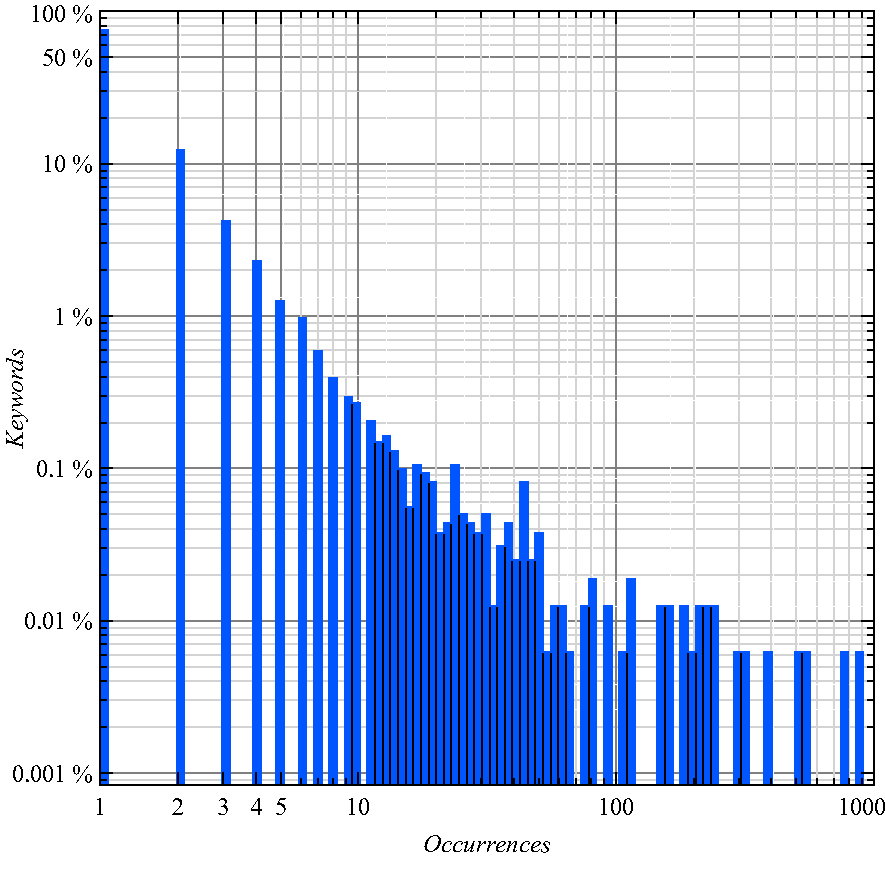
\includegraphics{images/keywords_clean_histogram_a.pdf}
\caption{Bla.}
\end{figure}

\begin{figure}
\centering
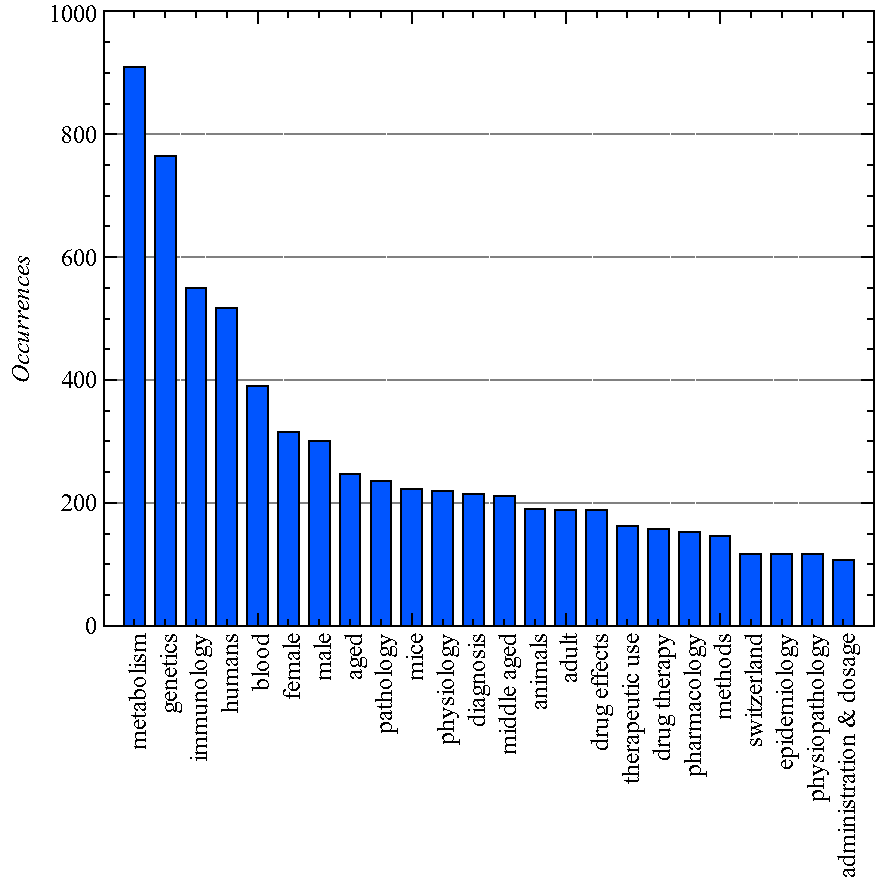
\includegraphics{images/keywords_clean_histogram_b.pdf}
\caption{Bla.}
\end{figure}

\hypertarget{reconciliation}{%
\paragraph{Reconciliation}\label{reconciliation}}

!! Mapping to controlled vocabularies; explain why this is necessary.

!! Does the OpenRefine project still exist? Export the list of changes!

\hypertarget{foreign-gold-standard}{%
\subsubsection{Foreign gold standard}\label{foreign-gold-standard}}

!! Todo: - Explain MeSH\\
- Explain how to get MeSH for subset of sample data set

\hypertarget{assessment}{%
\subsection{Assessment}\label{assessment}}

\hypertarget{precision-recall-f1-score}{%
\subsubsection{Precision, recall,
F1-score}\label{precision-recall-f1-score}}

!! Discussion of metrics

\hypertarget{annif-versus-native-gold-standard}{%
\subsubsection{Annif versus native gold
standard}\label{annif-versus-native-gold-standard}}

\hypertarget{yso}{%
\paragraph{YSO}\label{yso}}

\hypertarget{wikidata}{%
\paragraph{Wikidata}\label{wikidata}}

\hypertarget{annif-versus-foreign-gold-standard}{%
\subsubsection{Annif versus foreign gold
standard}\label{annif-versus-foreign-gold-standard}}

\hypertarget{digression-truth-conditions-for-indexing}{%
\subsubsection{Digression: truth-conditions for
indexing}\label{digression-truth-conditions-for-indexing}}

(Correspondence theory of indexing: subject term T fits text X iff text
X is about T) \#\#\# Targets !! Find out what I meant here.

\hypertarget{analysis-2}{%
\subsubsection{Analysis}\label{analysis-2}}

\hypertarget{discussion}{%
\subsection{Discussion}\label{discussion}}

\hypertarget{outlook}{%
\section{Outlook}\label{outlook}}

\hypertarget{refinement}{%
\subsection{Refinement}\label{refinement}}

\hypertarget{implementation-strategy}{%
\subsection{Implementation strategy}\label{implementation-strategy}}

\hypertarget{other-use-cases}{%
\subsection{Other use cases}\label{other-use-cases}}

\hypertarget{conclusion}{%
\section{Conclusion}\label{conclusion}}

\hypertarget{appendix}{%
\section{Appendix}\label{appendix}}

\hypertarget{bibliography}{%
\section{Bibliography}\label{bibliography}}

\hypertarget{refs}{}
\begin{CSLReferences}{1}{0}
\leavevmode\hypertarget{ref-Golub.2016}{}%
Golub, Koraljka, Dagobert Soergel, George Buchanan, Douglas Tudhope,
Marianne Lykke, and Debra Hiom. 2016. {``A Framework for Evaluating
Automatic Indexing or Classification in the Context of Retrieval.''}
\emph{Journal of the Association for Information Science and Technology}
67 (1): 3--16. \url{https://doi.org/10.1002/asi.23600}.

\leavevmode\hypertarget{ref-Louis.2013}{}%
Louis, Annie, and Ani Nenkova. 2013. {``Automatically Assessing Machine
Summary Content Without a Gold Standard.''} \emph{Computational
Linguistics} 39 (2): 267--300.
\url{https://doi.org/10.1162/COLI\%7B/textunderscore\%20\%7Da\%7B/textunderscore\%20\%7D00123}.

\leavevmode\hypertarget{ref-Parke.2013}{}%
Parke, Carol. 2013. \emph{Essential First Steps to Data Analysis:
Scenario-Based Examples Using SPSS}. Thousand Oaks: {SAGE Publications}.
\url{https://doi.org/10.4135/9781506335148}.

\leavevmode\hypertarget{ref-Stokhof.2011}{}%
Stokhof, Martin, and Michiel van Lambalgen. 2011. {``Abstractions and
Idealisations: The Construction of Modern Linguistics.''}
\emph{Theoretical Linguistics} 37 (1-2): 1--26.
\url{https://doi.org/10.1515/thli.2011.001}.

\leavevmode\hypertarget{ref-UniversitatBasel.2021}{}%
Universität Basel. n.d. {``Research Database of the University of Basel
User Manual.''} Edited by Universität Basel.

\end{CSLReferences}
